\section{RAVEN Concepts}
\label{sec:RAVENconcept}
In this section, we will introduce the main concepts that are behind the design of raven framework:
\begin{itemize}
    \item \textit{RAVEN input components}: Section ~\ref{sub:InputStructure} provides a brief introduction of the input components, introducing
    A detailed explanation of the input structure and keywords is reported in the user manual ~\cite{RAVENuserManual}.
    \item \textit{RAVEN entities}: Section ~\ref{sub:EntitiesAndFlow} is aimed to provide an overview on how the different objects in
    RAVEN can interact with each other, generating the user-dependent analysis flow
\end{itemize}
\subsection{Raven Input Components}
\label{sub:InputStructure}
The RAVEN code does not have a fixed calculation flow, since all of its basic
objects can be combined in order to create a user-defined calculation flow.
%
Thus, its input, eXtensible Markup Language (XML) format, is organized in different XML blocks, each with a
different functionality. For more information about XML, please click on the link:
\href{https://www.w3schools.com/xml/default.asp}{\textbf{XML tutorial}}.
%
\\The main input blocks are as follows:
\begin{itemize}
  \item \xmlNode{Simulation}: The root node containing the
  entire input, all of
  the following blocks fit inside the \emph{Simulation} block.
  %
  \item \xmlNode{RunInfo}: Specifies the calculation
  settings (number of parallel simulations, etc.).
  %
  \item \xmlNode{Files}: Specifies the files to be
  used in the calculation.
  %
  \item \xmlNode{Distributions}: Defines distributions
  needed for describing parameters, etc.
  %
  \item \xmlNode{Samplers}: Sets up the strategies used for
  exploring an uncertain domain.
  %
  \item \xmlNode{DataObjects}: Specifies internal data objects
  used by RAVEN.
  %
  \item \xmlNode{Databases}: Lists the HDF5 databases used
  as input/output to a
  RAVEN run.
  %
  \item \xmlNode{OutStreams}: Visualization and
  Printing system block.
  %
  \item \xmlNode{Models}: Specifies codes, ROMs,
  post-processing analysis, etc.
  %
  \item \xmlNode{Functions}: Details interfaces to external
  user-defined functions and modules. The user will be building and/or running.
  %
  \item \xmlNode{VariableGroups}: Creates a collection of variables.
  %
  \item \xmlNode{Optimizers}: Performs the driving of a specific goal function over
  the model for value optimization.
  %
  \item \xmlNode{Metrics}: Calculate the distance values among points and histories.
  %
  \item \xmlNode{Steps}: Combines other blocks to detail a
  step in the RAVEN workflow including I/O and computations to be performed.
  %
\end{itemize}

Each of these blocks are explained in dedicated sections of the user manual ~\cite{RAVENuserManual}. In this guide,
we will only show how to use these components to build the analysis flow, and we recommend the user to check the user
manual ~\cite{RAVENuserManual} for the detailed descriptions.
%
\\In addition, RAVEN allows the user to load any external input file that contains the required XML nodes into the RAVEN main input
file, and provide the standard XML comments, using\verb|<!--| and \verb|-->|. For example, one can use the following template to load
the \xmlNode{Distributions} from file `Distributions.xml'.
%
\begin{lstlisting}[style=XML,morekeywords={node,xmlToLoad}]
<Simulation verbosity='all'>
  ...
  <!-- An Example Comment -->
  <Steps verbosity='debug'>
    ...
  </Steps>
  ...
  <ExternalXML node='Distributions' xmlToLoad='path_to_folder/Distributions.xml'/>
  ...
</Simulation>
\end{lstlisting}
%
RAVEN also allows the user to control the level of output to the user interface by using \xmlAttr{verbosity} system. These settings can be
declared globally as attributes in the \xmlNode{Simulation} node, or locally in each block node as shown in above template.
The verbosity levels are
\begin{itemize}
\item \xmlString{silent} - Only simulation-breaking errors are displayed.
\item \xmlString{quiet} - Errors as well as warnings are displayed.
\item \xmlString{all} (default) - Errors, warnings, and messages are displayed.
\item \xmlString{debug} - For developers. All errors, warnings, messages, and debug messages are displayed.
\end{itemize}
%
\subsection{RAVEN Entities and Analysis Flow}
\label{sub:EntitiesAndFlow}
In the RAVEN code the number and types of possible analyses is potentially large (it is customization to many problem types).
Each basic action (sampling, printing, etc.) is encapsulated in
a dedicated object (named ``\textbf{Entity}''). Each object is inactive till it is connected with
other objects in order to perform a more complex process. For example,
the \textit{Sampler} entity, aimed to employ a perturbation action, becomes active only in case
it gets associated with a \textit{Model}, that is the internal representation of a physical model (e.g.,a system code).
\\RAVEN provides support for several \textbf{Entities}, which branch in several different categories/algorithms:
\begin{itemize}
  \item \textit{\xmlNode{RunInfo}}:
    \\The RunInfo \textbf{Entity} is an information container which describes how the overall computation should
      be performed. This \textbf{Entity}  accepts several input settings that define how to drive the calculation and set up,
      when needed, particular settings for the machine the code needs to run on (queue system, if not Portable Batch System-PBS, etc.).
  \item \textit{\xmlNode{Files}}:
  \\ The Files \textbf{Entity}  defines any files that might be needed within the RAVEN run. This could include inputs to the
      Model, pickled ROM files, or Comma Separated Value (CSV) files for post-processors, to name a few.
  \item \textit{\xmlNode{DataObjects}}:
    \\The DataObjects system is a container of data objects of various types that can be constructed during the execution of
    desired calculation flow. These data objects can be used as input or output for a particular \textit{Model}
     \textbf{Entity}. Currently RAVEN supports the following data types, each with a particular conceptual meaning:
     \begin{itemize}
        \item \textit{PointSet} is a collection of individual objects, each describing the state of the system at
                                a certain point (e.g. in time). It can be considered a mapping between multiple
                                            sets of parameters in the input space and the resulting sets of outcomes in the output space
                                            at a particular point (e.g., in time).
        \item \textit{HistorySet} is a collection of individual objects, each describing the temporal evolution of the
                                  state of the system within a certain input domain. It can be considered a mapping between
                                               multiple sets of parameters in the input space and the resulting sets of temporal evolution
                                               in the output space.
     \end{itemize}
     The DataObjects represent the preferred way to transfer the information coming from a Model (e.g., the driven code) to
      all the other RAVEN systems (e.g., Out-Stream system, Reduced Order Modeling component, etc.).
  \item \textit{\xmlNode{Databases}}:
      \\ RAVEN provides the capability to store and retrieve data to/from an external database. Currently RAVEN supports
       only a database type called \textit{HDF5}. This database, depending on the data format it is receiving, will
       organize itself in a ``parallel'' or ``hierarchical'' fashion. The user can create as many database \textbf{Entities} as needed.
  \item \textit{\xmlNode{Samplers}}:
  \\ The Samplers  \textbf{Entity} is the container of all the algorithms designed to perform the perturbation of the input space.
      The Samplers can be categorized into three main classes:
      \begin{itemize}
        \item  \textit{Forward}. Sampling strategies that do not leverage the information coming from already evaluated
        realizations in the input space. For example, Monte-Carlo, Stratified (LHS), Grid, Response Surface, Factorial Design,
        Sparse Grid, etc.
        \item  \textit{Adaptive}. Sampling strategies that take advantages of the information coming from already evaluated
        realizations of the input space, adapting the sampling strategies to key figures of merits. For example, Limit Surface
        search, Adaptive HDMR, etc.
        \item \textit{Dynamic Event Tree}. Sampling strategies that perform the exploration of the input space based on the
        dynamic evolution of the system, employing branching techniques. For example, Dynamic Event Tree, Hybrid
        Dynamic Event Tree, etc.
      \end{itemize}
  \item \textit{\xmlNode{OutStreams}}:
  \\ The OutStreams node is the \textbf{Entity} used for data exporting and dumping. The OutStreams support
   2 actions:
      \begin{itemize}
       \item \textit{Print}. This Out-Stream is able to print out (in a Comma Separated Value format) all the information
         contained in:
         \begin{itemize}
          \item DataObjects
          \item Reduced Order Models.
         \end{itemize}
       \item \textit{Plot}. This Out-Stream is able to plot 2-Dimensional, 3-Dimensional, 4-Dimensional (using color
       mapping) and 5-Dimensional (using marker size). Several types of plot are available, such as scatter, line, surfaces,
       histograms, pseudo-colors, contours, etc.
      \end{itemize}
  \item \textit{\xmlNode{Distributions}}:
  \\ The Distributions \textbf{Entity} is the container of all the stochastic representations of random variables. Currently,
  RAVEN supports:
      \begin{itemize}
       \item \textit{1-Dimensional} continuous and discrete distributions, such as Normal, Weibull, Binomial, etc.
       \item \textit{N-Dimensional} distributions, such as Multivariate Normal, user-inputted N-Dimensional distributions.
      \end{itemize}
  \item \textit{\xmlNode{Models}}:
  \\ The Models \textbf{Entity}  represents the projection from the input to the output space. Currently, RAVEN defines the
  following sub-categories:
      \begin{itemize}
       \item \textit{Code}, the sub-~\textbf{Entity} that represent the driven code, through external code interfaces (see~\cite{RAVENuserManual})
       \item  \textit{ExternalModel}, the sub-~\textbf{Entity} that represents a physical or mathematical model that is
       directly implemented by the user in a Python module
      \item \textit{ROM}, the sub-~\textbf{Entity} that represent the Reduced Order Model, interfaced with several algorithms
       \item \textit{PostProcessor}, the sub-~\textbf{Entity} that is used to perform action on data, such as computation of
       statistical moments, correlation matrices, etc.
      \end{itemize}
      The Model \textbf{Entity} can be seen as a transfer function between the input and output space.
  \item \textit{\xmlNode{Functions}}:
   \\ The Functions \textbf{Entity} is the container of all the user-defined functions, such as Goal Functions in adaptive
   sampling strategies, etc.
  \item \textit{\xmlNode{VariableGroups}}:
    \\ The VariableGroups \textbf{Entity} allows the user to create a collection of variables instead of re-listing all
    the variables in places throughout the input file, such as DataObjects, ROMs, and ExternalModels. Each entry in the
    VariableGroup block has a distinct name and list of each constituent variable in the group. Alternatively, set operations
    can be used to construct variable groups from other variable groups. In this case, the dependent groups and the
    base group on which operations should be performed must be listed.  The following types of set operations are included in RAVEN:
    \begin{itemize}
      \item \texttt{+}, Union, the combination of all variables in the \xmlString{base} set and listed set,
      \item \texttt{-}, Complement, the relative complement of the listed set in the \xmlString{base} set,
      \item \texttt{\^}, Intersection, the variables common to both the \xmlString{base} and listed set,
      \item \texttt{\%}, Symmetric Difference, the variables in only either the \xmlString{base} or listed set,
      but not both.
    \end{itemize}
    Multiple operations can be performed by separating them with commas in the text of the group node.  In the
    event the listed set is a single variable, it will be treated like a set with a single entry.
    %
    When using the variable groups in a node, they can be listed alone or as part of a comma-separated list.  The
    variable group name will only be substituted in the text of nodes, not attributes or tags.
  \item \textit{\xmlNode{Optimizers}}:
    \\ The optimizer is another important entity in the RAVEN framework. It performs the driving of a specific goal function
    over the model for value optimization. The difference between an optimizer and a sampler is that the former does not require
    sampling over a distribution, although certain specific optimizers may utilize stochastic approach to locate the optimality.
    The optimizers currently available in RAVEN can be categorized into the following class(es):
    \begin{itemize}
      \item \textbf{Gradient Based Optimizer}
    \end{itemize}
  \item \textit{\xmlNode{Metrics}}:
   \\
    The Metrics block allows the user to specify the similarity/dissimilarity metrics to be used in specific clustering algorithms available in RAVEN.
    These metrics are used to calculate the distance values among points and histories.
    The data mining algorithms in RAVEN which accept the definition of a metric are the following:
    \begin{itemize}
      \item DBSCAN 
      \item Affinity Propagation 
    \end{itemize}
    Both of these algorithms can take as input an $N \times N$ square matrix $D=[d_{ij}]$ where each element $d_{ij}$ of $D$ is the distance between 
    element $i$ $(i=1,\ldots,N)$ and $j$
    $(j=1,\ldots,N)$.

    Available metrics are as follows:
    \begin{itemize}
      \item Minkowski
    \end{itemize}
\end{itemize}
All these action-objects are combined together to create a peculiar analysis flow, which is specified
by the user in an additional \textbf{Entity} named \textit{\xmlNode{Steps}} (see Fig.~\ref{fig:ravenStructure}).
This \textbf{Entity} represents the core of the analysis, since it is the location where the multiple objects get
finally linked in order to perform a combined action on a certain \textit{Model} (see Fig.~\ref{fig:ExampleStepEntity}).
Currently, RAVEN supports the following types of \textit{\xmlNode{Steps}}:
\begin{itemize}
  \item \textit{SingleRun}, perform a single run of a model
  \item \textit{MultiRun}, perform multiple runs of a model
  \item \textit{RomTrainer}, perform the training of a Reduced Order Model (ROM)
  \item \textit{PostProcess}, post-process data or manipulate RAVEN entities
  \item \textit{IOStep}, step aimed to perform multiple actions:
  \begin{itemize}
    \item construct/update a Database from a DataObjects and vice-versa
    \item construct/update a Database or a DataObjects object from CSV files
    \item stream the content of a Database or a DataObjects out through an OutStream
    \item store/retrieve a ROM to/from an external File using Pickle module of Python
  \end{itemize}
\end{itemize}
\begin{figure}[h!]
  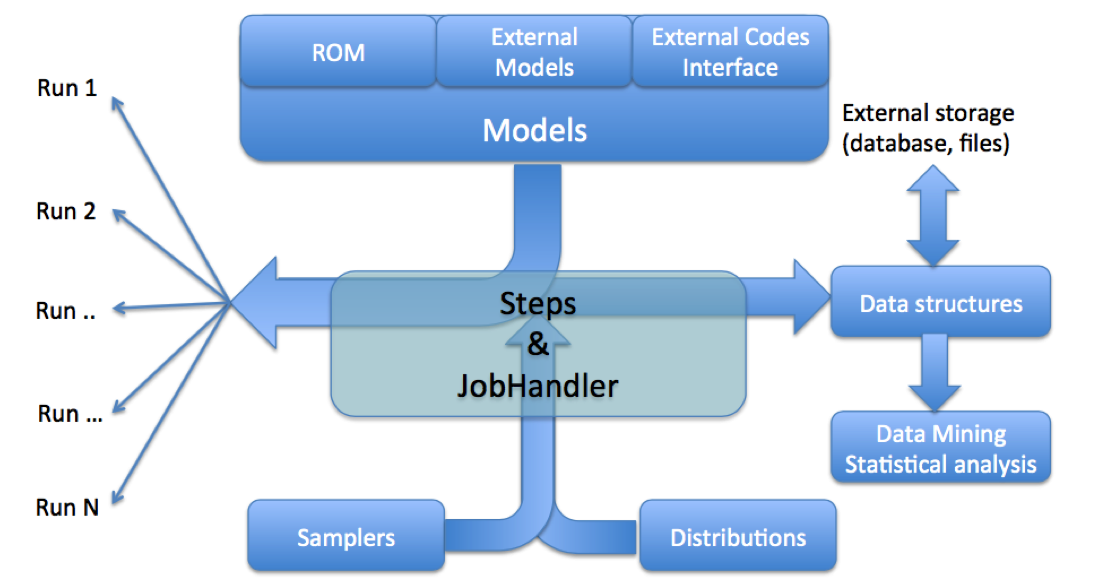
\includegraphics[width=\textwidth]{pics/ravenStructure.png}
  \caption{RAVEN structures}
  \label{fig:ravenStructure}
\end{figure}
\begin{figure}[h!]
  \includegraphics[scale=1]{pics/ExampleStepEntity.png}
  \caption{Example of the Steps \textbf{Entity}  and its connection in the input file.}
  \label{fig:ExampleStepEntity}
\end{figure}
